\documentclass[12pt]{book}
\usepackage[utf8]{inputenc}
\usepackage[T1]{fontenc}
\usepackage{amsmath, amssymb, amsthm}
\usepackage{graphicx}
\usepackage{hyperref}
\usepackage{geometry}
\usepackage{tikz}
\usetikzlibrary{graphs, positioning}

\newenvironment{encadre}
  {\begin{center}\begin{tabular}{|p{0.9\textwidth}|}\hline}
  {\\\hline\end{tabular}\end{center}}
  
\geometry{margin=2.5cm}
\setcounter{secnumdepth}{2}
\setcounter{tocdepth}{2}


% Métadonnées
\title{Géométrie des Données et Apprentissage Machine}
\author{Youssef MESRI - MINES Paris - PSL}
\date{\today}

\begin{document}


\frontmatter
\maketitle
	\tableofcontents

\mainmatter

\chapter{Géométrie des Données}
\section{Introduction}
La géométrie des données est une discipline fondamentale pour comprendre et exploiter la structure cachée des données modernes, souvent de très haute dimension. Ce livre propose une introduction détaillée aux concepts clés, illustrés par des exemples, des démonstrations et des exercices corrigés.\par


Les données modernes, issues de domaines variés (images, sons, textes, signaux), sont généralement représentées dans des espaces vectoriels de grande dimension ($\mathbb{R}^d$ avec $d \gg 1$). Pourtant, ces données possèdent souvent une structure intrinsèque de faible dimension, appelée \textbf{variété}.\par

	\textbf{Exemple :} Les images de chiffres manuscrits (base MNIST) sont des vecteurs de dimension 784, mais l'ensemble des images possibles se répartit sur une variété de dimension beaucoup plus faible (environ 10).\par

Ce chapitre est organisé en plusieurs sections, chacune abordant un aspect fondamental de la géométrie des données et de l'apprentissage sur variétés :
\begin{itemize}
	\item Malédiction de la dimension et concentration des distances
	\item Variétés et distances géodésiques
	\item Réduction de dimension : PCA, Isomap, Diffusion Maps, t-SNE
	\item Applications pratiques et exercices
\end{itemize}

\section{Malédiction de la dimension et concentration des distances}
\subsection{Explosion dimensionnelle}
Lorsque la dimension $d$ augmente, le volume de l'espace croît exponentiellement. Dans un cube unité $[0,1]^d$, la majeure partie du volume se concentre près des bords.\par

Les distances entre points deviennent moins discriminantes :
\begin{align*}
d_{\min} &= \min_{i \neq j} \|x_i - x_j\|, \\
d_{\max} &= \max_{i \neq j} \|x_i - x_j\|.
\end{align*}
On observe que :
\[
\lim_{d \to \infty} \frac{d_{\max} - d_{\min}}{d_{\min}} \to 0.
\]
	\textbf{Conséquence :} toutes les distances deviennent presque égales !\par

\subsection{Concentration des distances}
La distance au carré entre deux points aléatoires $x, y \in [0,1]^d$ s'écrit :
\[
S_d = \|x-y\|_2^2 = \sum_{i=1}^d (x_i-y_i)^2.
\]
L'espérance et la variance de $S_d$ croissent avec $d$, mais la dispersion relative décroît comme $1/\sqrt{d}$.\par

	\textbf{Interprétation :} En grande dimension, toutes les distances se ressemblent (concentration autour de la moyenne). Les méthodes classiques basées sur la distance (kNN, clustering) deviennent inefficaces.\par

\subsection{Démonstration mathématique}
Soient $U,V \sim \mathcal{U}[0,1]$ indépendants. Posons $X=(U-V)^2$.\par
	\textbf{Espérance :} $\mathbb{E}[X]=\frac{1}{6}$\par
	\textbf{Moment d'ordre 4 :} $\mathbb{E}[(U-V)^4]=\frac{1}{15}$\par
	\textbf{Variance :} $\operatorname{Var}(X)=\frac{7}{180}$\par

Pour $d$ dimensions, $S_d = \sum_{i=1}^d X_i$ avec $X_i$ i.i.d.\par
	\textbf{Espérance :} $\mathbb{E}[S_d]=d\mu$\par
	\textbf{Variance :} $\operatorname{Var}(S_d)=d\sigma^2$\par
	\textbf{Coefficient de variation :} $\frac{\sqrt{d\sigma^2}}{d\mu} = \frac{C}{\sqrt{d}}$\par

\subsection{Exercice}
	\textbf{Montrer que la différence de deux variables uniformes sur $[0,1]$ suit une loi triangulaire sur $[-1,1]$.}

	\textbf{Corrigé :} La densité de $Z = U - V$ est donnée par :
\[
f_Z(z) = \begin{cases} 1+z, & -1\le z < 0, \\
1-z, & 0\le z \le 1, \\
0, & \text{sinon}.\end{cases}
\]

\subsection{Conséquences pratiques}
Les méthodes classiques basées sur des distances euclidiennes deviennent inefficaces en grande dimension. Il est nécessaire d'utiliser des méthodes exploitant la structure intrinsèque des données (géométrie des données).\par


\section{Variétés et distances géodésiques}
\subsection{Qu'est-ce qu'une variété ?}
Une \textbf{variété} est un espace qui, localement, ressemble à un espace euclidien de dimension plus faible. Les données réelles, bien que plongées dans un espace de grande dimension, sont souvent contraintes par des relations internes qui les font se répartir sur une variété de dimension intrinsèque $k \ll d$.\par

	\textbf{Exemple :} Les images de chiffres manuscrits, bien que décrites par 784 pixels, sont générées par un nombre limité de facteurs (forme, épaisseur, inclinaison, etc.), ce qui réduit la dimension effective de l'ensemble des images possibles.\par

\subsection{Distance euclidienne vs distance géodésique}
La \textbf{distance euclidienne} mesure le plus court chemin dans l'espace ambiant $\mathbb{R}^d$. Sur une variété courbe, cette distance peut être trompeuse : deux points proches sur la variété peuvent être éloignés euclidiennement si la variété est repliée.\par

La \textbf{distance géodésique} est la longueur du plus court chemin sur la variété elle-même. Elle capture la vraie proximité intrinsèque des données.\par

	\textbf{Illustration :} Sur un "Swiss Roll" (rouleau suisse), la distance euclidienne entre deux points sur des tours différents est grande, alors que la distance géodésique (le long du rouleau) est plus courte.\par

\subsection{Conséquences pour l'apprentissage}
Les méthodes d'apprentissage doivent tenir compte de la structure de la variété pour être efficaces. Les algorithmes de réduction de dimension (Isomap, Diffusion Maps, t-SNE) cherchent à préserver les distances géodésiques ou la structure locale de la variété.\par

\subsection{Exercice}
	\textbf{Exercice :} Sur un Swiss Roll généré en 3D, comparez la distance euclidienne et la distance géodésique entre deux points situés sur des tours différents.\par

	\textbf{Corrigé :} La distance euclidienne ignore la structure du rouleau et peut relier deux points à travers l'espace, alors que la distance géodésique suit la surface du rouleau, respectant la structure intrinsèque des données.

\section{Réduction de dimension : PCA, Isomap, Diffusion Maps, t-SNE}
\subsection{Pourquoi réduire la dimension ?}
La réduction de dimension vise à représenter des données de grande dimension dans un espace de plus faible dimension, tout en préservant leur structure essentielle. Cela facilite la visualisation, l'analyse et l'apprentissage automatique.\par

\subsection{Analyse en Composantes Principales (PCA)}
\subsubsection{Définition et principe}
L'Analyse en Composantes Principales (PCA) est une méthode linéaire de réduction de dimension qui consiste à projeter les données sur les axes de plus grande variance. Elle permet de simplifier la structure des données tout en conservant l'information essentielle.

	\textbf{Objectif :} Trouver les directions principales (axes) qui capturent le plus de variance dans les données.

\subsubsection{Algorithme de la PCA}
\begin{enumerate}
	\item Centrer les données : soustraire la moyenne de chaque variable.
	\item Calculer la matrice de covariance $\Sigma$ :
		\[
		\Sigma = \frac{1}{n}\sum_{i=1}^n (x_i - \mu)(x_i - \mu)^T
		\]
	\item Calculer les valeurs propres et vecteurs propres de $\Sigma$.
	\item Sélectionner les $k$ plus grandes valeurs propres et leurs vecteurs associés.
	\item Projeter les données sur les $k$ axes principaux.
\end{enumerate}

	\textbf{Remarque :} La décomposition en valeurs singulières (SVD) de la matrice des données $X$ est une alternative efficace pour calculer la PCA.

\subsubsection{Exemple numérique}
\begin{itemize}
	\item Données simulées $X \in \mathbb{R}^{100\times 5}$.
	\item Calcul de la matrice de covariance, valeurs propres et projection sur les deux premières composantes principales.
	\item Visualisation : les données se concentrent le long des directions principales.
\end{itemize}

\subsubsection{Applications}
\begin{itemize}
	\item Visualisation de données haute dimension (ex : MNIST en 2D ou 3D).
	\item Prétraitement pour l'apprentissage automatique.
	\item Compression et débruitage.
\end{itemize}

\subsubsection{Exercices}
\begin{itemize}
	\item Appliquer la PCA sur un jeu de données simulé et visualiser les deux premières composantes.
	\item Calculer la variance expliquée par chaque composante et choisir le nombre optimal de dimensions.
	\item Utiliser la SVD pour réaliser la PCA sur des données réelles.
\end{itemize}

\subsection{Isomap}

\subsubsection{Définition et principe}
Isomap (Isometric Mapping) est une méthode non linéaire de réduction de dimension qui vise à préserver les distances géodésiques entre les points d'une variété plongée dans un espace de haute dimension. Elle étend la méthode MDS (Multidimensional Scaling) aux variétés non linéaires.

	\textbf{Objectif :} Reconstituer la structure intrinsèque des données en utilisant les distances le long de la variété (géodésiques) plutôt que les distances euclidiennes.

\subsubsection{Algorithme Isomap}
\begin{enumerate}
	\item Construire le graphe de voisinage ($k$-NN ou $\epsilon$-voisinage).
	\item Calculer les plus courts chemins entre tous les points (algorithme de Dijkstra ou Floyd-Warshall) pour approximer les distances géodésiques.
	\item Appliquer la MDS (décomposition spectrale de la matrice de distances) pour obtenir une représentation en dimension réduite.
\end{enumerate}

\subsubsection{Exemple : Swiss Roll}
\begin{itemize}
	\item Générer un jeu de données 3D enroulé (Swiss Roll).
	\item PCA ne parvient pas à "dérouler" la structure.
	\item Isomap reconstitue correctement la structure 2D sous-jacente.
\end{itemize}

\subsubsection{Applications}
\begin{itemize}
	\item Visualisation de variétés non linéaires.
	\item Analyse de la structure intrinsèque des données.
\end{itemize}

\subsubsection{Exercices}
\begin{itemize}
	\item Implémenter Isomap sur un Swiss Roll et visualiser la représentation 2D obtenue.
	\item Comparer les résultats d'Isomap et de PCA sur des données simulées.
	\item Étudier l'influence du paramètre $k$ sur la qualité de la reconstruction.
\end{itemize}

\subsection{Diffusion Maps}

\subsubsection{Définition et principe}
Diffusion Maps est une méthode non linéaire de réduction de dimension qui exploite la notion de diffusion sur un graphe de voisinage pour révéler la structure globale et multi-échelle des données. Elle repose sur l'analyse spectrale du laplacien du graphe construit à partir des données.

	\textbf{Objectif :} Capturer la connectivité et la structure intrinsèque des données, même en présence de bruit ou de distributions complexes.

\subsubsection{Algorithme Diffusion Maps}
\begin{enumerate}
	\item Construire le graphe de voisinage (pondéré par une fonction de similarité, ex : $W_{ij} = \exp(-\|x_i-x_j\|^2/\varepsilon)$).
	\item Calculer la matrice de transition $P = D^{-1}W$, où $D$ est la matrice de degré.
	\item Calculer les valeurs propres $\lambda_1, \lambda_2, ...$ et vecteurs propres $\psi_i$ de $P$.
	\item Représenter chaque point $x$ par le vecteur $(\lambda_1^t\psi_1(x), ..., \lambda_k^t\psi_k(x))$ pour une certaine échelle $t$.
\end{enumerate}

\subsubsection{Exemple : Séparation de groupes}
\begin{itemize}
	\item Appliquer Diffusion Maps sur des données connectées par des chemins complexes.
	\item Permet de séparer des groupes de données difficilement distinguables par des méthodes classiques.
\end{itemize}

\subsubsection{Applications}
\begin{itemize}
	\item Analyse de la connectivité globale des données.
	\item Visualisation et clustering robuste au bruit.
	\item Étude de phénomènes dynamiques (ex : diffusion sur réseaux).
\end{itemize}

\subsection{Exercices}
\begin{itemize}
	\item Implémenter Diffusion Maps sur un Swiss Roll bruité et comparer avec Isomap.
	\item Tester différents paramètres ($\varepsilon$, $t$) et observer leur influence sur la représentation.
	\item Visualiser les vecteurs propres et interpréter leur signification géométrique.
\end{itemize}

\subsection{t-SNE}

\subsubsection{Définition et principe}
t-SNE (t-distributed Stochastic Neighbor Embedding) est une méthode non linéaire de réduction de dimension et de visualisation, conçue pour préserver la structure locale des données. Elle est particulièrement efficace pour représenter des clusters et des groupes dans des données complexes.

	\textbf{Objectif :} Représenter fidèlement les voisins proches et révéler la structure locale des données en 2D ou 3D.

\subsubsection{Algorithme t-SNE}
\begin{enumerate}
	\item Calculer les similarités locales entre points dans l'espace original (probabilités $p_{ij}$).
	\item Placer les points dans l'espace réduit et définir des similarités $q_{ij}$ (loi t de Student).
	\item Minimiser la divergence de Kullback-Leibler entre $p_{ij}$ et $q_{ij}$ par descente de gradient.
	\item Ajuster les paramètres (perplexité, learning rate) pour optimiser la séparation des clusters.
\end{enumerate}

\subsubsection{Exemple : Visualisation MNIST}
\begin{itemize}
	\item Appliquer t-SNE sur les images MNIST pour obtenir une carte 2D où chaque chiffre forme un groupe distinct.
	\item Comparer la séparation des classes avec PCA et Isomap.
\end{itemize}

\subsubsection{Applications}
\begin{itemize}
	\item Visualisation intuitive de données complexes.
	\item Analyse exploratoire et détection de clusters.
	\item Prétraitement pour le clustering ou la classification.
\end{itemize}

\subsubsection{Exercices}
\begin{itemize}
	\item Appliquer t-SNE sur différents jeux de données et analyser la structure obtenue.
	\item Étudier l'influence de la perplexité et du learning rate sur la visualisation.
	\item Comparer t-SNE avec PCA et Diffusion Maps sur des données simulées et réelles.
\end{itemize}

\subsection{Exercices}
\begin{itemize}
	\item Appliquer la PCA, Isomap et t-SNE sur le jeu de données MNIST. Comparer les visualisations obtenues.
	\item Sur un Swiss Roll, comparer les résultats de PCA, Isomap et Diffusion Maps.
\end{itemize}

\section{Applications pratiques et exercices}

\subsection{TP et exercices avancés}
\subsubsection{TP1 : Visualisation et réduction de dimension sur MNIST}
\begin{itemize}
	\item Appliquer PCA, Isomap, Diffusion Maps et t-SNE sur le jeu de données MNIST.
	\item Visualiser les résultats en 2D et 3D, analyser la séparation des classes.
	\item Corrigé : PCA sépare globalement, t-SNE isole les clusters, Isomap et Diffusion Maps révèlent la structure intrinsèque.
\end{itemize}

\subsubsection{TP2 : Swiss Roll et reconstruction de variétés}
\begin{itemize}
	\item Générer un Swiss Roll synthétique en 3D.
	\item Appliquer PCA, Isomap et Diffusion Maps, comparer la capacité à "dérouler" la structure.
	\item Corrigé : PCA échoue, Isomap et Diffusion Maps réussissent à retrouver la structure 2D.
\end{itemize}

\subsubsection{TP3 : Étude de la concentration des distances}
\begin{itemize}
	\item Simuler des points dans $[0,1]^d$ pour différentes valeurs de $d$.
	\item Calculer la distance moyenne et l'écart-type, observer la concentration.
	\item Corrigé : l'écart relatif décroît avec $d$, illustrant la malédiction de la dimension.
\end{itemize}

\subsubsection{TP4 : Paramètres et robustesse des méthodes}
\begin{itemize}
	\item Étudier l'influence des paramètres ($k$ pour Isomap, $\varepsilon$ et $t$ pour Diffusion Maps, perplexité pour t-SNE).
	\item Tester sur des données bruitées ou incomplètes.
	\item Corrigé : certains paramètres rendent les méthodes plus robustes ou sensibles au bruit.
\end{itemize}

\subsection{Exercices avancés}
\begin{itemize}
	\item Implémenter Isomap et Diffusion Maps sur des jeux de données réels (ex : images, signaux).
	\item Comparer les avantages et limites de chaque méthode selon la nature des données.
	\item Discuter les applications possibles en IA, physique, biologie.
\end{itemize}

%==============================
\chapter{Graphes et diffusion sur données}


\section{Introduction et construction de graphes}
La représentation des relations locales entre points d'un nuage de données est essentielle pour de nombreuses méthodes modernes d'apprentissage et d'analyse. Les graphes permettent de modéliser ces relations via différentes constructions :
\begin{itemize}
  \item \textbf{k-NN graph} : chaque point est relié à ses $k$ plus proches voisins, ce qui garantit une connectivité locale contrôlée.
  \item \textbf{$\varepsilon$-graph} : relie tous les points dont la distance est inférieure à $\varepsilon$, le nombre de voisins varie selon la densité locale.
\end{itemize}
Les graphes peuvent être pondérés pour refléter la similarité entre points :
\[
  w_{ij} = \exp\Big(-\frac{\|x_i - x_j\|^2}{2\sigma^2}\Big)
\]
La pondération permet de capturer la force de connexion locale et prépare le graphe pour les méthodes spectrales.

\begin{encadre}
\textbf{Exercice :}
Construisez un graphe k-NN et un $\varepsilon$-graph sur un jeu de données 2D (ex : spirale, cercles imbriqués). Visualisez les différences de connectivité et discutez l'impact du choix de $k$ et $\varepsilon$.
\end{encadre}

\begin{figure}[h!]
\centering
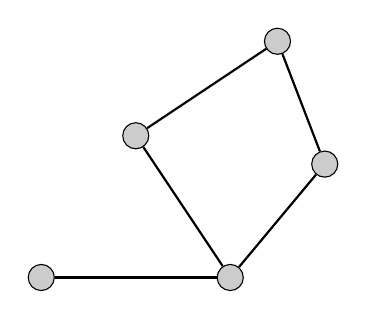
\begin{tikzpicture}[scale=1.2]
% Graphe k-NN
\foreach \i/\x/\y in {1/0/0,2/2/0,3/1/1.5,4/3/1.2,5/2.5/2.5} {
  \node[circle,draw,fill=black!20] (P\i) at (\x,\y) {};
}
% k-NN edges
\draw[thick] (P1) -- (P2);
\draw[thick] (P2) -- (P4);
\draw[thick] (P2) -- (P3);
\draw[thick] (P3) -- (P5);
\draw[thick] (P4) -- (P5);
\end{tikzpicture}
\caption{Exemple de graphe k-NN sur des points 2D}
\end{figure}

\begin{figure}[h!]
\centering
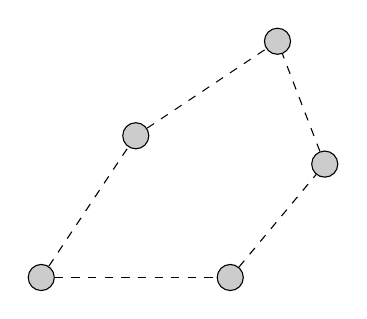
\begin{tikzpicture}[scale=1.2]
% Graphe epsilon
\foreach \i/\x/\y in {1/0/0,2/2/0,3/1/1.5,4/3/1.2,5/2.5/2.5} {
  \node[circle,draw,fill=black!20] (P\i) at (\x,\y) {};
}
% epsilon edges
\draw[dashed] (P1) -- (P3);
\draw[dashed] (P2) -- (P4);
\draw[dashed] (P3) -- (P5);
\draw[dashed] (P4) -- (P5);
\draw[dashed] (P1) -- (P2);
\end{tikzpicture}
\caption{Exemple de graphe $\varepsilon$ sur des points 2D}
\end{figure}

\section{Laplacien de graphe : définitions et interprétations}
Soit $G=(V,E,W)$ un graphe pondéré avec matrice de poids $W$ et matrice de degrés $D$ :
\[
  D_{ii} = \sum_j w_{ij}
\]
Le Laplacien non normalisé est $L = D - W$. Les variantes normalisées sont :
\[
  L_{\text{sym}} = D^{-1/2} L D^{-1/2}, \quad L_{\text{rw}} = D^{-1} L
\]
Le Laplacien est semi-défini positif, et son vecteur propre associé à $\lambda_0=0$ est constant. Il joue un rôle central dans la diffusion et la réduction de dimension.

\subsection{Interprétation et propriétés}
Le Laplacien est l'analogue discret du Laplacien continu sur une variété. Il mesure la variation d'une fonction $f$ sur le graphe :
\[
  f^\top L f = \frac{1}{2} \sum_{i,j} w_{ij} (f_i - f_j)^2
\]
Un petit $f^\top L f$ indique que $f$ varie peu entre voisins fortement connectés. Les vecteurs propres associés aux plus petites valeurs propres capturent la structure globale du graphe (Eigenmaps), utiles pour la réduction de dimension et le clustering spectral.

\begin{encadre}
\textbf{Exercice :}
Pour un graphe simple (ex : chaîne, cycle), calculez le Laplacien et ses valeurs propres. Interprétez les vecteurs propres en termes de structure du graphe.
\end{encadre}

\begin{figure}[h!]
\centering
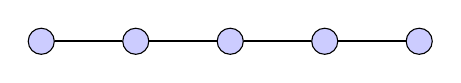
\begin{tikzpicture}[scale=1.2]
% Graphe chaîne
\foreach \i/\x in {1/0,2/1,3/2,4/3,5/4} {
  \node[circle,draw,fill=blue!20] (N\i) at (\x,0) {};
}
\foreach \i in {1,2,3,4} {
  \draw[thick] (N\i) -- (N\the\numexpr\i+1\relax);
}
\end{tikzpicture}
\caption{Graphe chaîne : illustration du Laplacien}
\end{figure}

\section{Diffusion sur graphe et noyau de chaleur}
La diffusion sur graphe s'appuie sur la matrice de transition $P = D^{-1} W$ (random walk). La propagation d'une fonction $f$ se fait par :
\[
  f(t+1) = P f(t)
\]
Le noyau de chaleur discret est donné par :
\[
  H_t = e^{-tL} \approx \sum_{k=0}^{n-1} e^{-t \lambda_k} \phi_k \phi_k^\top
\]
Il mesure la diffusion de la chaleur entre points après un temps $t$, révélant les structures multi-échelles et la proximité entre points.

\begin{encadre}
\textbf{Exemple :}
Initialisez la chaleur sur un noeud d'un graphe et simulez la diffusion pour différents temps $t$. Observez la propagation et discutez l'effet de la topologie (bottleneck, clusters).
\end{encadre}

\begin{figure}[h!]
\centering
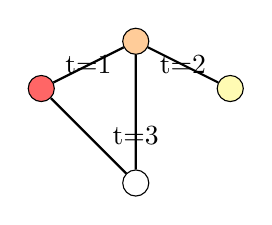
\begin{tikzpicture}[scale=1.2]
% Diffusion sur graphe
\node[circle,draw,fill=red!60] (A) at (0,0) {};
\node[circle,draw,fill=orange!40] (B) at (1,0.5) {};
\node[circle,draw,fill=yellow!30] (C) at (2,0) {};
\node[circle,draw,fill=white] (D) at (1,-1) {};
\draw[thick] (A) -- (B) -- (C);
\draw[thick] (B) -- (D);
\draw[thick] (A) -- (D);
\node at (0.5,0.25) {t=1};
\node at (1.5,0.25) {t=2};
\node at (1,-0.5) {t=3};
\end{tikzpicture}
\caption{Diffusion multi-échelle sur un graphe}
\end{figure}

\section{Apprentissage semi-supervisé sur graphe}
L'objectif est de propager des labels connus sur un sous-ensemble de points vers l'ensemble du graphe. On résout l'équation de Poisson discrète :
\[
  L f = 0 \quad \text{sur les points non étiquetés}
\]
avec conditions de Dirichlet sur les points étiquetés. La solution pratique consiste à résoudre le système linéaire restreint :
\[
  L_{uu} f_u = - L_{u\ell} Y_\ell
\]
Les labels se diffusent le long des arêtes pondérées, permettant la classification semi-supervisée.

\begin{encadre}
\textbf{TP : Classification semi-supervisée sur graphes}
Utilisez un sous-ensemble étiqueté du jeu MNIST pour propager les labels sur le graphe k-NN. Comparez la performance selon le nombre de labels connus et la structure du graphe.
\end{encadre}

\begin{figure}[h!]
\centering
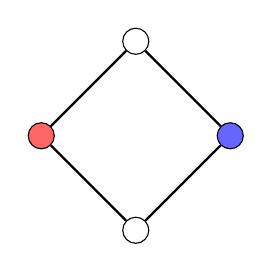
\begin{tikzpicture}[scale=1.2]
% Propagation de labels
\node[circle,draw,fill=red!60] (R) at (0,0) {};
\node[circle,draw,fill=blue!60] (B) at (2,0) {};
\node[circle,draw,fill=white] (U1) at (1,1) {};
\node[circle,draw,fill=white] (U2) at (1,-1) {};
\draw[thick] (R) -- (U1) -- (B);
\draw[thick] (R) -- (U2) -- (B);
\end{tikzpicture}
\caption{Propagation de labels sur un graphe}
\end{figure}

\section{Courbure de graphe et topologie intuitive}
La courbure discrète mesure comment les voisins d’un noeud sont connectés entre eux. Les points de "bottleneck" relient deux clusters et ralentissent la diffusion. Les valeurs propres du Laplacien capturent la topologie : modes lents pour les grandes structures, modes rapides pour les détails locaux. Cette analyse guide la détection de communautés et la compréhension des structures locales et globales.

\begin{encadre}
\textbf{Exercice :}
Construisez un graphe avec deux clusters reliés par un bottleneck. Simulez la diffusion et observez la lenteur de la propagation entre clusters.
\end{encadre}

\begin{figure}[h!]
\centering
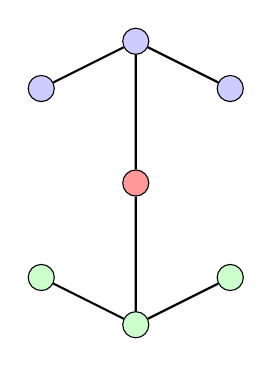
\begin{tikzpicture}[scale=1.2]
% Bottleneck
\node[circle,draw,fill=blue!20] (A1) at (0,1) {};
\node[circle,draw,fill=blue!20] (A2) at (1,1.5) {};
\node[circle,draw,fill=blue!20] (A3) at (2,1) {};
\node[circle,draw,fill=green!20] (B1) at (0,-1) {};
\node[circle,draw,fill=green!20] (B2) at (1,-1.5) {};
\node[circle,draw,fill=green!20] (B3) at (2,-1) {};
\node[circle,draw,fill=red!40] (M) at (1,0) {};
\draw[thick] (A1) -- (A2) -- (A3);
\draw[thick] (B1) -- (B2) -- (B3);
\draw[thick] (A2) -- (M);
\draw[thick] (B2) -- (M);
\end{tikzpicture}
\caption{Bottleneck : deux clusters reliés par un point central}
\end{figure}

\section{Applications pratiques}
\subsection{Classification de digits (MNIST)}
On construit un graphe k-NN ou $\varepsilon$-graph à partir des images, pondère les arêtes par similarité, puis applique Laplacian Eigenmaps ou diffusion pour réduire la dimension. Les labels connus sont propagés par Poisson discrete.

\subsection{Segmentation d'image}
Les pixels sont les noeuds du graphe, les arêtes reflètent le voisinage spatial et la similarité de couleur. La diffusion ou Poisson discrete permet de propager des labels initiaux pour obtenir une segmentation cohérente.

\subsection{Applications modernes}
\textbf{NLP} : graphes de mots ou documents, arêtes pondérées par similarité sémantique, diffusion pour classification ou extraction de communautés.
\textbf{Bioinformatique} : réseaux de gènes ou protéines, propagation de labels, clustering, analyse multi-échelle.

\section{Résumé du chapitre}
\begin{itemize}
  \item Construction de graphes : k-NN, $\varepsilon$-graph, pondérés
  \item Laplacien : définitions, interprétations, Eigenmaps
  \item Diffusion et noyau de chaleur : distances multi-échelles
  \item Poisson discrete : propagation de labels
  \item Courbure et topologie : bottlenecks, structures locales et globales
  \item Exemples : classification, segmentation
  \item Applications : NLP, bioinformatique
\end{itemize}

\begin{encadre}
\textbf{Pour aller plus loin :}
- Explorez les graphes orientés, les graphes dynamiques et les applications en réseaux sociaux.
- Testez la robustesse des méthodes spectrales face au bruit et aux données manquantes.
- Comparez diffusion, random walk et autres méthodes de propagation sur différents types de graphes.
\end{encadre}


\chapter{Deep Learning sur Graphes et Variétés}

\section{Motivation et limites des modèles classiques}
Les modèles classiques d'apprentissage (MLP, CNN) sont conçus pour des données euclidiennes (vecteurs, images 2D) et supposent une structure régulière. Ils présentent plusieurs limites :
\begin{itemize}
	\item Non différentiables ou difficilement applicables sur graphes/variétés
	\item Difficulté à capturer les relations locales et globales non régulières
	\item Scalabilité limitée pour des structures complexes
\end{itemize}

\begin{center}
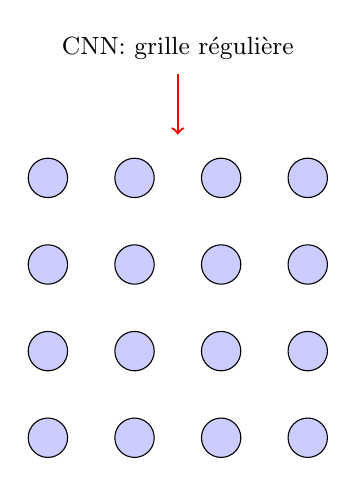
\begin{tikzpicture}[scale=1.1]
	% Grille euclidienne (CNN)
	\foreach \x in {0,1,2,3} {
		\foreach \y in {0,1,2,3} {
			\node[draw, circle, fill=blue!20, minimum size=0.5cm] at (\x,\y) {};
		}
	}
	\draw[thick,red,->] (1.5,4.2) -- (1.5,3.5);
	\node at (1.5,4.5) {\small CNN: grille régulière};
\end{tikzpicture}
\hspace{1cm}
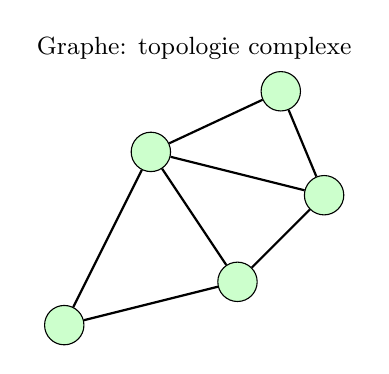
\begin{tikzpicture}[scale=1.1]
	% Graphe irrégulier
	\node[draw, circle, fill=green!20, minimum size=0.5cm] (A) at (0,0) {};
	\node[draw, circle, fill=green!20, minimum size=0.5cm] (B) at (2,0.5) {};
	\node[draw, circle, fill=green!20, minimum size=0.5cm] (C) at (1,2) {};
	\node[draw, circle, fill=green!20, minimum size=0.5cm] (D) at (3,1.5) {};
	\node[draw, circle, fill=green!20, minimum size=0.5cm] (E) at (2.5,2.7) {};
	\draw[thick] (A) -- (B) -- (C) -- (D) -- (E) -- (C);
	\draw[thick] (A) -- (C);
	\draw[thick] (B) -- (D);
	\node at (1.5,3.2) {\small Graphe: topologie complexe};
\end{tikzpicture}
\end{center}

\begin{encadre}
	\textbf{Exemple :}
\begin{itemize}
	\item Les CNN ne peuvent pas propager l'information entre voisins arbitraires sur un graphe
	\item Les MLP traitent des vecteurs fixes, sans tenir compte de la topologie
\end{itemize}
\end{encadre}

\section{Principe du Message Passing}
Pour traiter des données structurées (graphes, variétés), on utilise le principe du \textbf{message passing} : chaque nœud met à jour sa représentation en agrégeant les informations de ses voisins.
\begin{align*}
	h_i^{(l+1)} = \text{UPDATE}\Big(h_i^{(l)}, \text{AGGREGATE}(\{h_j^{(l)} : j \in \mathcal{N}(i)\})\Big)
\end{align*}
\begin{itemize}
	\item \textbf{Message} : $m_{ij} = \phi(h_i^{(l)}, h_j^{(l)}, e_{ij})$
	\item \textbf{Agrégation} : somme/moyenne/max des messages
	\item \textbf{Mise à jour} : $h_i^{(l+1)} = \psi(h_i^{(l)}, m_i)$
\end{itemize}

\begin{encadre}
	extbf{À retenir :}
\begin{itemize}
  \item Le message passing généralise la convolution aux structures non régulières (graphes, maillages).
  \item Il permet de capturer l'information locale et globale dans des réseaux complexes.
\end{itemize}
\end{encadre}

\begin{encadre}
	extbf{Question de réflexion :}
\begin{itemize}
  \item Pourquoi la convolution classique ne fonctionne-t-elle pas sur un graphe ?
  \item Quelles sont les limites du message passing pour des graphes très grands ou très hétérogènes ?
\end{itemize}
\end{encadre}

\begin{center}
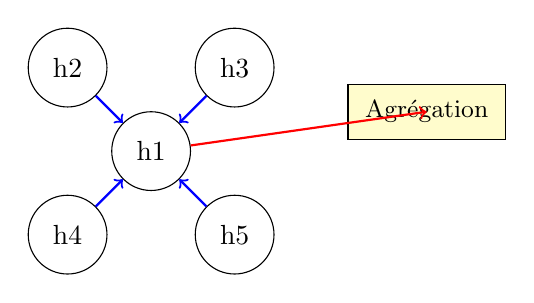
\begin{tikzpicture}[node distance=1.5cm, every node/.style={circle,draw,minimum size=1cm}]
	\node (h1) {h1};
	\node (h2) [above left of=h1] {h2};
	\node (h3) [above right of=h1] {h3};
	\node (h4) [below left of=h1] {h4};
	\node (h5) [below right of=h1] {h5};
	\foreach \i in {h2,h3,h4,h5} {\draw[->,thick,blue] (\i) -- (h1);}
	\node[draw,rectangle,fill=yellow!20,minimum width=2cm,minimum height=0.7cm] at (3.5,0.5) {\small Agrégation};
	\draw[->,thick,red] (h1) -- (3.5,0.5);
\end{tikzpicture}
\end{center}

\begin{encadre}
	\textbf{Illustration : propagation de messages}
\begin{center}
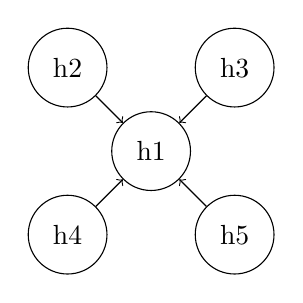
\begin{tikzpicture}[node distance=1.5cm, every node/.style={circle,draw,minimum size=1cm}]
	\node (h1) {h1};
	\node (h2) [above left of=h1] {h2};
	\node (h3) [above right of=h1] {h3};
	\node (h4) [below left of=h1] {h4};
	\node (h5) [below right of=h1] {h5};
	\foreach \i in {h2,h3,h4,h5} {\draw[->] (\i) -- (h1);}
\end{tikzpicture}
\end{center}
\end{encadre}

\section{Exemple concret}
Supposons un graphe de personnes, chaque nœud ayant un attribut (âge). À chaque étape, chaque personne met à jour son âge en prenant la moyenne pondérée de son âge et de ceux de ses voisins :
\begin{align*}
	h_i^{(l+1)} = \tfrac{1}{2} h_i^{(l)} + \tfrac{1}{2} \frac{1}{|\mathcal{N}(i)|} \sum_{j \in \mathcal{N}(i)} h_j^{(l)}
\end{align*}
Après plusieurs itérations, chaque nœud possède une représentation influencée par ses voisins proches et éloignés.

\begin{encadre}
	extbf{Application pratique :}
\begin{itemize}
	\item Propagation d'information dans les réseaux sociaux (ex : diffusion d'une opinion ou d'une rumeur).
	\item Recommandation personnalisée : chaque utilisateur agrège les préférences de ses voisins dans le graphe d'interactions.
\end{itemize}
\end{encadre}

\section{Graph Convolutional Network (GCN)}
Le GCN (Kipf \& Welling 2017) généralise la convolution aux graphes :

\begin{align*}
	H^{(l+1)} = \sigma \Big( \tilde{D}^{-1/2} \tilde{A} \tilde{D}^{-1/2} H^{(l)} W^{(l)} \Big)
\end{align*}
\begin{encadre}
	extbf{À retenir :}
\begin{itemize}
	\item Le GCN applique une normalisation symétrique pour stabiliser l'apprentissage.
	\item Il permet de traiter des graphes non réguliers et d'apprendre des représentations structurées.
\end{itemize}
\end{encadre}
où $\tilde{A} = A + I$ (adjacence avec boucles), $\tilde{D}$ (degrés), $H^{(l)}$ (représentations), $W^{(l)}$ (poids).
\begin{encadre}
	\textbf{Exemple PyTorch Geometric :}
\begin{verbatim}
import torch
import torch.nn.functional as F
from torch_geometric.nn import GCNConv

class GCN(torch.nn.Module):
		def __init__(self, in_dim, hid_dim, out_dim):
				super().__init__()
				self.conv1 = GCNConv(in_dim, hid_dim)
				self.conv2 = GCNConv(hid_dim, out_dim)

		def forward(self, x, edge_index):
				x = F.relu(self.conv1(x, edge_index))
				x = self.conv2(x, edge_index)
				return F.log_softmax(x, dim=1)
\end{verbatim}
\end{encadre}

\section{Graph Attention Network (GAT)}
Le GAT introduit un mécanisme d'attention pour pondérer l'importance des voisins :
\begin{align*}
	\alpha_{ij} = \frac{ \exp \big( \text{LeakyReLU}(a^\top [W h_i \| W h_j]) \big) }
												{ \sum_{k \in \mathcal{N}(i)} \exp \big( \text{LeakyReLU}(a^\top [W h_i \| W h_k]) \big) }
\end{align*}
\begin{align*}
	h_i^{(l+1)} = \sigma \left( \sum_{j \in \mathcal{N}(i)} \alpha_{ij} W h_j \right)
\end{align*}

\begin{encadre}
	extbf{À retenir :}
\begin{itemize}
  \item Le GAT apprend à pondérer chaque voisin selon son importance pour la tâche.
  \item Il est particulièrement utile pour des graphes hétérogènes ou des relations complexes.
\end{itemize}
\end{encadre}

\section{Comparaison GCN vs GAT}
\begin{itemize}
	\item \textbf{GCN} : normalisation fixe, voisins traités uniformément, simplicité
	\item \textbf{GAT} : pondération apprise, plus flexible, coût de calcul plus élevé
\end{itemize}

\begin{encadre}
	extbf{Question de réflexion :}
\begin{itemize}
  \item Dans quels cas préférer GAT à GCN ?
  \item Quels sont les avantages et inconvénients de l'attention sur les graphes ?
\end{itemize}
\end{encadre}

\begin{center}
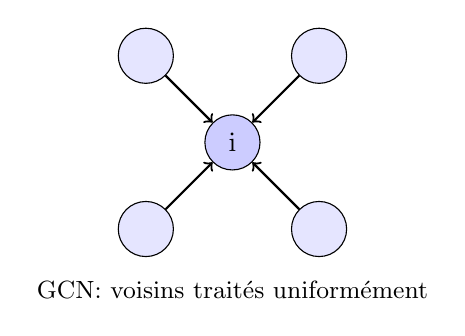
\begin{tikzpicture}[scale=1.1]
	% GCN: voisins uniformes
	\node[draw, circle, fill=blue!20, minimum size=0.7cm] (A) at (0,0) {i};
	\foreach \x/\y in {1/1,1/-1,-1/1,-1/-1} {
		\node[draw, circle, fill=blue!10, minimum size=0.7cm] (N\x\y) at (\x,\y) {};
		\draw[->,thick] (N\x\y) -- (A);
	}
	\node at (0,-1.7) {\small GCN: voisins traités uniformément};
\end{tikzpicture}
\hspace{1cm}
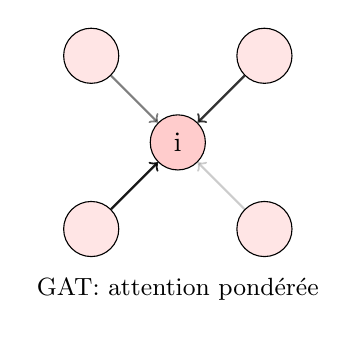
\begin{tikzpicture}[scale=1.1]
	% GAT: attention
	\node[draw, circle, fill=red!20, minimum size=0.7cm] (A) at (0,0) {i};
	\foreach \x/\y/\c in {1/1/0.8,1/-1/0.2,-1/1/0.5,-1/-1/0.9} {
		\node[draw, circle, fill=red!10, minimum size=0.7cm] (N\x\y) at (\x,\y) {};
		\draw[->,thick,opacity=\c] (N\x\y) -- (A);
	}
	\node at (0,-1.7) {\small GAT: attention pondérée};
\end{tikzpicture}
\end{center}

\section{Deux approches : Spectral vs Spatial}
\begin{itemize}
	\item \textbf{Spectral} : décomposition spectrale du Laplacien, analyse fréquentielle
	\item \textbf{Spatial} : agrégation locale des voisins, message passing
\end{itemize}

\section{Applications de l’IA géométrique}
\begin{itemize}
	\item Physique computationnelle : simulation moléculaire, dynamique des particules
	\item Biologie structurale : protéines, réseaux de gènes
	\item IA générative : diffusion sur variétés et graphes
\end{itemize}

\begin{encadre}
	extbf{À retenir :}
\begin{itemize}
  \item Les GNN sont utilisés dans des domaines variés où la structure des données est essentielle.
  \item Ils permettent de modéliser des interactions complexes et des phénomènes dynamiques.
\end{itemize}
\end{encadre}

\section{Outils Python pour l’IA géométrique}
\begin{itemize}
	\item \textbf{PyTorch Geometric (PyG)} : bibliothèque modulaire basée sur PyTorch
	\item \textbf{DGL (Deep Graph Library)} : efficace, multi-backend
	\item \textbf{Spektral} : intégré à TensorFlow/Keras
\end{itemize}
\begin{encadre}
	\textbf{Exemple DGL :}
\begin{verbatim}
import dgl
import torch.nn as nn
import torch.nn.functional as F
from dgl.nn import GraphConv

class GCN(nn.Module):
		def __init__(self, in_dim, hid_dim, out_dim):
				super().__init__()
				self.conv1 = GraphConv(in_dim, hid_dim)
				self.conv2 = GraphConv(hid_dim, out_dim)

		def forward(self, g, features):
				x = F.relu(self.conv1(g, features))
				x = self.conv2(g, x)
				return F.log_softmax(x, dim=1)
\end{verbatim}
\end{encadre}

\begin{encadre}
	\textbf{Exemple Spektral :}
\begin{verbatim}
import tensorflow as tf
from spektral.layers import GCNConv

class GCN(tf.keras.Model):
		def __init__(self, out_dim):
				super().__init__()
				self.conv1 = GCNConv(16, activation="relu")
				self.conv2 = GCNConv(out_dim, activation="softmax")

		def call(self, inputs):
				x, a = inputs
				x = self.conv1([x, a])
				return self.conv2([x, a])
\end{verbatim}
\end{encadre}

\section{Conclusion et perspectives}
Le deep learning géométrique permet de traiter des données sur graphes, maillages et variétés, en exploitant les relations locales et topologiques complexes. Les techniques clés incluent le message passing, les GNN (GCN, GAT), l'apprentissage spectral et spatial, et l'exploitation de la structure pour l'IA générative et scientifique. Les outils Python modernes (PyTorch Geometric, DGL, Spektral) facilitent l'implémentation de ces modèles. Les applications couvrent la physique, la biologie et l'IA générative. Ouverture : optimisation, IA générative avancée, intégration avec HPC.
\chapter{Topologie des données, variétés et transport optimal}

\section{Plan du module}
\begin{itemize}
	\item Introduction à la topologie des données
	\item Variétés riemanniennes
	\item Transport optimal
	\item Applications à l’IA générative
	\item TP : Mapper (KeplerMapper), mini-projet transport optimal (POT library)
\end{itemize}

\section{Topologie des données}
Pour étudier la forme globale des données (trous, cycles, composantes), on utilise des techniques comme :
\begin{enumerate}
	\item \textbf{Mapper} : visualisation simplifiée d’un nuage de points
	\item \textbf{Persistent Homology} : détection de features topologiques robustes
\end{enumerate}
\begin{encadre}
	extbf{Diagramme de persistance :}
Barres représentant la durée de vie des composantes.\par
	exttt{Points $\to$ Graphe simplicial $\to$ Filtration $\to$ Barcodes}
\begin{itemize}
	\item Chaque barre = un trou ou composante connectée
	\item Longue barre $\to$ feature robuste
	\item Courte barre $\to$ bruit
\end{itemize}
\end{encadre}

\section{Variétés riemanniennes}
Une variété lisse $(\mathcal{M}, g)$ avec métrique $g$ définit longueur et angles.\par
La distance géodésique $d_\mathcal{M}(x,y)$ est la longueur minimale d’un chemin sur $\mathcal{M}$.\par
	extbf{Exemples :} sphère, tore, espace de rotations SO(3).\par
	extbf{Applications :} données sur sphère, pose 3D, embedding non-linéaire.

\section{Transport optimal}
Comparer deux distributions $\mu$ et $\nu$ avec la distance de Wasserstein :
\begin{align*}
	W_p(\mu, \nu) = \Bigg( \inf_{\gamma \in \Pi(\mu, \nu)} \int \|x - y\|^p d\gamma(x,y) \Bigg)^{1/p}
\end{align*}
\begin{itemize}
	\item Comparaison distributions réelles vs générées
	\item Génération de données réalistes avec structures géométriques
\end{itemize}

\section{Applications à l’IA générative}
\begin{itemize}
	\item Score-based diffusion : génération par gradient de log-densité
	\item Transport optimal : mesurer distances entre distributions générées et réelles
	\item Topologie persistante : régulariser génération pour préserver cycles/structures
	\item Graphes et variétés : génération de molécules, maillages 3D, images structurées
\end{itemize}

\section{TP : Mapper et transport optimal}
\begin{encadre}
	extbf{TP Mapper (KeplerMapper)} :
Visualiser la structure globale d’un nuage de points avec Mapper. Utiliser la bibliothèque KeplerMapper pour explorer les cycles et composantes.
\end{encadre}
\begin{encadre}
	extbf{Mini-projet transport optimal (POT library)} :
Implémenter la comparaison de distributions et le calcul de la distance de Wasserstein avec la bibliothèque POT. Appliquer à des données réelles ou simulées.
\end{encadre}

\section{Synthèse}
\begin{itemize}
	\item Topologie : Mapper, Persistent Homology → analyser la forme globale des données
	\item Géométrie avancée : variétés riemanniennes et distances géodésiques
	\item Transport optimal : distance de Wasserstein pour comparer distributions
	\item Applications IA générative : score-based diffusion, OT, régularisation topologique
\end{itemize}

\end{document}